\documentclass[10pt,leqno]{amsart}
\usepackage{graphicx}
\baselineskip=16pt

\usepackage{indentfirst,csquotes}

\topmargin= .5cm
\textheight= 22.5cm
\textwidth= 32cc
\baselineskip=16pt

\evensidemargin= .9cm
\oddsidemargin= .9cm

\usepackage{amssymb,amsthm,amsmath}
\usepackage{xcolor,paralist,hyperref,titlesec,fancyhdr,etoolbox}
\newtheorem{theorem}{Theorem}[]
\newtheorem{definition}[theorem]{Definition}
\newtheorem{example}[theorem]{Example}
\newtheorem{lemma}[theorem]{Lemma}
\newtheorem{proposition}[theorem]{Proposition}
\newtheorem{corollary}[theorem]{Corollary}
\newtheorem{conjecture}[theorem]{Conjecture}

\titleformat{\section}[display]{\normalfont\huge\bfseries\centering}{\centering\chaptertitlename\thechapter}{10pt}{\Large}
\titlespacing*{\section}{0pt}{0ex}{0ex}

\hypersetup{ colorlinks=true, linkcolor=black, filecolor=black, urlcolor=black }
\def\proof{\noindent {\it Proof. $\, $}}
\def\endproof{\hfill $\Box$ \vskip 5 pt }

% --- Additions to the proposal template (report only) -----------------------
\usepackage{booktabs}
\usepackage{placeins}   % \FloatBarrier keeps figures inside their own section
% The template's \titleformat breaks \section in amsart (\chaptertitlename is
% undefined), so headings follow the proposal's bold run-in style.
\newcommand{\heading}[1]{\medskip\noindent\textbf{#1}\par}
\newcommand{\E}{\mathbb{E}}
\newcommand{\Q}{\mathbb{Q}}
% Option-chain experiment: generated by heston/report_assets.py (never typed by hand).
\newcommand{\DeltaDate}{2024-06-03}
\newcommand{\DeltaGapAtm}{-0.024}
\newcommand{\ExDate}{2023-03-23}
\newcommand{\ExExpiry}{2023-04-27}
\newcommand{\ExF}{17\,186}
\newcommand{\ExHedge}{+469.5}
\newcommand{\ExK}{17\,200}
\newcommand{\ExNet}{+34.1}
\newcommand{\ExNetBp}{+19.8}
\newcommand{\ExPay}{715.0}
\newcommand{\ExPrem}{279.6}
\newcommand{\ExStory}{The index rises, so the call finishes worth 715.0 points, which the desk pays to the buyer; the long-futures hedge earns 469.5 points back:}
\newcommand{\FitBad}{72}
\newcommand{\FitMedian}{0.73}
\newcommand{\HedgeSDBS}{61.2}
\newcommand{\HedgeSDH}{71.3}
\newcommand{\HedgeSDMV}{55.9}
\newcommand{\HedgeSDNone}{264}
\newcommand{\HvsBSTest}{+36}
\newcommand{\HvsBSTestZ}{4.4}
\newcommand{\KappaBoundPct}{70}
\newcommand{\MVvsBSAll}{-8}
\newcommand{\MVvsBSAllZ}{-0.8}
\newcommand{\MVvsBSCovid}{-63}
\newcommand{\MVvsBSCovidZ}{-4.4}
\newcommand{\MVvsBSExCovid}{+8}
\newcommand{\MVvsBSExCovidZ}{1.3}
\newcommand{\MVvsBSTest}{-17}
\newcommand{\MVvsBSTestZ}{-1.3}
\newcommand{\MVvsHTest}{-39}
\newcommand{\MVvsHTestZ}{-3.6}
\newcommand{\NCovid}{113}
\newcommand{\NDays}{4\,031}
\newcommand{\NHedges}{3\,931}
\newcommand{\NOptionDays}{391\,792}
\newcommand{\NQuotes}{418\,345}
\newcommand{\PriceBSAtmAll}{3.87}
\newcommand{\PriceBSAtmTest}{3.89}
\newcommand{\PriceBSOwnAll}{1.11}
\newcommand{\PriceBSOwnTest}{1.14}
\newcommand{\PriceFlatOverHeston}{2.5}
\newcommand{\PriceHestonAll}{1.55}
\newcommand{\PriceHestonTest}{1.58}
\newcommand{\RhoMedian}{-0.40}
\newcommand{\SimCalHvsBS}{+10}
\newcommand{\SimCalMVFour}{73.9}
\newcommand{\SimCalMVWeek}{102.4}
\newcommand{\SimCalMVvsBS}{-5}
\newcommand{\SimCalParams}{(v_0,\kappa,\theta,\xi,\rho)=(0.021,\,15.0,\,0.024,\,1.38,\,-0.37)}
\newcommand{\SimCalSDBS}{81.1}
\newcommand{\SimCalSDMV}{79.2}
\newcommand{\SimTSHvsBS}{+8}
\newcommand{\SimTSMVFour}{30.2}
\newcommand{\SimTSMVWeek}{84.1}
\newcommand{\SimTSMVvsBS}{-2}
\newcommand{\SimTSSDBS}{45.4}
\newcommand{\SimTSSDMV}{44.8}
\newcommand{\StratBSDD}{$-$5.6}
\newcommand{\StratBSHighRet}{+0.17}
\newcommand{\StratBSRet}{+1.4}
\newcommand{\StratBSSharpe}{0.74}
\newcommand{\StratBSWorstDay}{$-$2.2}
\newcommand{\StratMVDD}{$-$4.1}
\newcommand{\StratMVHighRet}{$-$0.03}
\newcommand{\StratMVRet}{+1.2}
\newcommand{\StratMVSharpe}{0.62}
\newcommand{\StratMVSkipSharpe}{0.64}
\newcommand{\StratMVWorstDay}{$-$2.5}
\newcommand{\StratMeanGrossBS}{+12.4}
\newcommand{\StratMeanGrossMV}{+10.7}
\newcommand{\StratMeanNone}{$-$10.0}
\newcommand{\StratMeanNoneAbs}{10.0}
\newcommand{\StratNoneDD}{$-$36}
\newcommand{\StratNoneRet}{$-$1.8}
\newcommand{\StratPremium}{182}
\newcommand{\StratTurnMV}{1.7}
\newcommand{\SurfDateA}{2024-06-03}
\newcommand{\SurfDateB}{2020-03-18}
\newcommand{\XiMedian}{1.34}

% Time-series experiment: transcribed from the team's outputs (source note in the file).
% Numbers from the team's time-series experiment (rough Heston / classical Heston with
% parameters estimated from NIFTY and India VIX histories). TRANSCRIBED from the team PDF
% "heston_option_pricing.pdf" (17 Nov 2026, Tables 1-3, 12-13 and Sections 3.1.1-3.2.4),
% which reports the outputs of src/compare_models.py and related scripts in
% MACF244_heston_rough_all_code.zip. They are NOT regenerated by heston/report_assets.py.
% VERIFIED 19 Nov 2026: the team's full pipeline was re-run in a copy of the old repo
% (69 tests pass); every number below matches the fresh outputs
% (results/pricing_test/all_models.md, results/backtest_heston/hedging_error_es99_all_models.md,
% results/model_comparison/model_comparison_report.md, heston_params.json, rough_params.json),
% except the two simulation ES99 values, which the PDF gave as 473.1 / 631.4 and which we
% recomputed from the old project's results/discrete_rebalancing/per_path.npz
% (50,000 paths, every-step rebalancing, zero cost, ES = mean loss beyond the 99% quantile).
% Every time-series number in the report comes from this file only.
\newcommand{\TSAlpha}{0.555}
\newcommand{\TSHestonParams}{(\kappa,\theta,\xi,\rho)\approx(8.60,\,0.0337,\,0.341,\,-0.526)}
\newcommand{\TSDates}{1\,819}
\newcommand{\TSOptions}{46\,299}
\newcommand{\TSTrain}{2\,076}
\newcommand{\TSTest}{1\,914}
\newcommand{\TSRoughVsBSAtm}{-0.33}
\newcommand{\TSRoughVsBSAtmCI}{[-0.44,\,-0.24]}
\newcommand{\TSRoughVsBSAll}{-0.43}
\newcommand{\TSRoughVsBSAllCI}{[-0.61,\,-0.25]}
\newcommand{\TSRoughWinPct}{77}
\newcommand{\TSMVScoreDiff}{-2.6}
\newcommand{\TSMVScoreCI}{[-7.3,\,1.2]}
\newcommand{\TSMVESDiff}{-34.9}
\newcommand{\TSMVESCI}{[-70.2,\,7.1]}
\newcommand{\TSMVESRestr}{+6.1}
\newcommand{\TSMVESRestrCI}{[1.4,\,8.4]}
\newcommand{\TSRoughMVESRestr}{+22.5}
\newcommand{\TSRoughMVESRestrCI}{[6.0,\,32.6]}
\newcommand{\TSSimGKW}{473.5}
\newcommand{\TSSimBS}{626.0}

% -----------------------------------------------------------------------------

\begin{document}
\title[Heston and Rough Heston Hedging on NIFTY]{Heston and Rough Heston Option Pricing and Hedging: Evidence from NIFTY Options}
\author{MAC F244: Stochastic Calculus and Applications to Finance \\ Project Report}
\date{\today}
\maketitle
\vspace{-1.5em}

\let\thefootnote\relax
\footnotetext{MSC2020: Primary 91G20, Secondary 60H30.}

\bigskip

\heading{1. Problem and summary.}
\noindent Black--Scholes prices and hedges an option perfectly when volatility is constant. Real index volatility moves, is correlated with the index, and produces a volatility smile, so the market is incomplete and no stock-only hedge is perfect. We ask two practical questions on the NSE NIFTY 50 index, 2010--2026:
\begin{compactenum}
\item Do stochastic-volatility models, classical Heston and rough Heston, \emph{price} traded NIFTY options better than Black--Scholes?
\item Does the variance-minimising (minimum-variance) hedge of these models \emph{hedge} better than the Black--Scholes delta, and does the answer change in crises?
\end{compactenum}
We answer them with two complementary designs on real data:
\begin{compactitem}
\item \textbf{Experiment A (time-series inputs).} Model parameters are estimated from NIFTY and India VIX \emph{histories}, then used to price traded options and to hedge synthetic one-month calls with costs.
\item \textbf{Experiment B (option-chain calibration).} Classical Heston is re-calibrated \emph{every day} to the traded option chain (\NDays{} days, \NQuotes{} quotes) and tested strictly one day ahead, for pricing and for hedging traded calls with futures.
\end{compactitem}
\emph{Main findings.}
\begin{compactitem}
\item \textbf{Pricing.} With five parameters a day, calibrated Heston prices the next day's options with \PriceFlatOverHeston{} times smaller error than Black--Scholes with one volatility (RMSE \PriceHestonAll{} vs \PriceBSAtmAll{} vol points): it \emph{produces} the smile that Black--Scholes must be given. With only historical inputs, rough Heston prices traded calls best: its at-the-money error minus that of Black--Scholes at India VIX is $\TSRoughVsBSAtm$ vol points (95\% interval $\TSRoughVsBSAtmCI$), and it wins on \TSRoughWinPct\% of dates.
\item \textbf{Hedging.} The minimum-variance correction derived by Itô's formula matters: the plain Heston delta hedges worse than Black--Scholes (error variance $\HvsBSTest\%$), and the correction removes that loss (error variance $\MVvsHTest\%$ against the plain Heston delta). In the COVID-19 crash the minimum-variance hedge changed the error variance by $\MVvsBSCovid\%$ against Black--Scholes ($z=\MVvsBSCovidZ$), exactly when volatility moved most.
\item \textbf{The strongest benchmark.} Black--Scholes fed with each option's own implied volatility (yesterday's whole market smile) is still a slightly better pricer (\PriceBSOwnAll{}) and, outside COVID, an equally good hedge. A better price fit does not, by itself, give a better hedge.
\end{compactitem} A simulation in which Heston is exactly true explains why: there too the minimum-variance hedge improves on the Black--Scholes own-vol hedge by only a few percent ($\SimCalMVvsBS\%$ in variance), too little to detect in the real sample. Finally we turn the project into a strategy, selling hedged index options as an insurer would: with low costs the Heston-hedged book earns \StratMVRet\% of notional a year with Sharpe \StratMVSharpe{} in the test period, and its edge disappears at higher costs.

\heading{2. Models.}
\noindent Work under a pricing measure $\Q$ with zero interest rate, and let $F_t$ be the futures (forward) price of the index.

\emph{Black--Scholes and incompleteness.} If $dF_t=\sigma F_t\,dW_t$ with constant $\sigma$, Itô's formula applied to the call price $C(t,F)$ shows that holding $\Delta=C_F$ futures removes all risk; this is the martingale representation of the payoff with one Brownian motion. Once volatility is random and driven by a second Brownian motion, the option has risk that the futures cannot replicate.

\emph{Classical Heston (1993).} The variance $v_t$ is a mean-reverting square-root process,
\begin{equation}\label{eq:heston}
dF_t=\sqrt{v_t}\,F_t\,dW^1_t,\qquad dv_t=\kappa(\theta-v_t)\,dt+\xi\sqrt{v_t}\,dW^2_t,\qquad d\langle W^1,W^2\rangle_t=\rho\,dt .
\end{equation}
Here $\kappa$ is the speed of mean reversion, $\theta$ the long-run variance, $\xi$ the volatility of variance and $\rho<0$ the leverage correlation (the index falls when volatility rises), which creates the downside skew in implied volatility.

\emph{Rough Heston.} Empirically, log-volatility is much rougher than a Brownian path (Gatheral, Jaisson and Rosenbaum 2018). Rough Heston (El Euch and Rosenbaum 2018, 2019) keeps the Heston structure but lets the variance remember past shocks through a power-law weight:
\[
v_t=v_0+\int_0^t K(t-s)\Big[\lambda(\theta-v_s)\,ds+\nu\sqrt{v_s}\,dW^2_s\Big],\qquad K(u)=\frac{u^{\alpha-1}}{\Gamma(\alpha)},\quad \tfrac12<\alpha\le 1 .
\]
Recent shocks get large weight and old shocks fade slowly. At $\alpha=1$ the weight is constant and the model is classical Heston; smaller $\alpha$ means rougher volatility. From the variogram of NIFTY log range-volatility (training period) we estimate $\alpha\approx\TSAlpha$, that is, NIFTY volatility is rough.

\emph{Pricing.} Both models price a European call as
\[
C_0=F_0\,P_1-K\,P_2 ,
\]
where $P_2=\Q(F_T>K)$ is the exercise probability and $P_1$ is the same probability under the measure that uses the futures as numéraire. Both probabilities are obtained from the model's characteristic function by a one-dimensional Fourier integral (Gil-Pelaez 1951; Heston 1993). For Heston this function is explicit (we use the numerically stable form of Albrecher et al.\ 2007); for rough Heston it is computed numerically. We use the authors' published formulas and treat the rough pricer as a numerical tool.

\heading{3. The minimum-variance hedge.}
\noindent Let $C(t,F,v)$ be the call price under \eqref{eq:heston}. By Itô's formula the random part of $dC$ is
\[
dC=(\dots)\,dt+C_F\sqrt v\,F\,dW^1+C_v\,\xi\sqrt v\,dW^2 .
\]
Holding $\varphi$ futures leaves the residual $dC-\varphi\,dF$. Its variance is smallest for the ratio of covariations
\begin{equation}\label{eq:mv}
\varphi^{\mathrm{MV}}=\frac{d\langle C,F\rangle}{d\langle F\rangle}=\frac{C_F\,vF^2+C_v\,\rho\xi\,vF}{vF^2}=C_F+\frac{\rho\,\xi}{F}\,C_v ,
\end{equation}
because $d\langle F\rangle=vF^2dt$ and $d\langle F,v\rangle=\rho\xi vF\,dt$. The first term is the Heston delta, which treats variance as fixed. The second hedges the part of the variance move that is predictable from the index: since $\rho<0$ and $C_v>0$, it \emph{lowers} the hedge of a call. Formula \eqref{eq:mv} is the stock-only projection of the option on the futures (the Galtchouk--Kunita--Watanabe decomposition), and its empirical analogue is the Hull--White (2017) minimum-variance delta. Rough Heston has a hedge of the same form, with $C_v$ replaced by the price sensitivity to the whole future variance curve; we use it as computed by the team's code. Figure~\ref{fig:delta} shows the size of the correction.

\begin{figure}[ht]
\centering
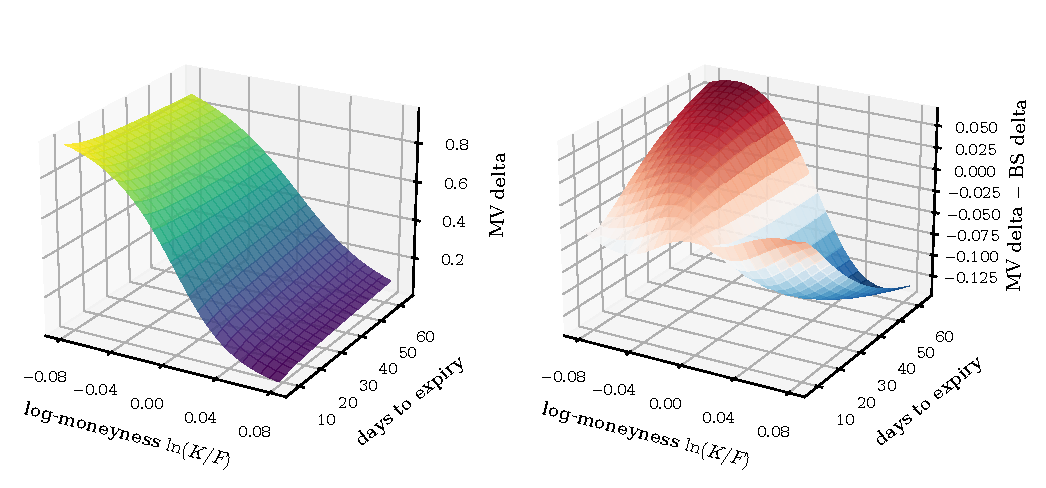
\includegraphics[width=\textwidth]{figures/delta_surface}
\caption{Classical Heston minimum-variance delta (left) and its difference from a Black--Scholes delta at the model's average volatility (right), across log-moneyness and days to expiry, for the parameters calibrated on \DeltaDate. The correction is of order $0.05$--$0.1$ in delta.}\label{fig:delta}
\end{figure}

\heading{4. Data.}
\noindent All data are free and public.
\begin{compactitem}
\item \textbf{Options and futures:} NSE F\&O daily bhavcopy (nsearchives.nseindia.com), NIFTY rows, 19 July 2010 to 21 October 2026. The format changed to UDiFF on 8 July 2024; both formats are normalised to one schema. A price counts only if the contract traded that day.
\item \textbf{Index and volatility index:} NIFTY 50 daily closes (niftyindices.com) and India VIX (NSE; Yahoo Finance series checked against NSE).
\item \textbf{Checks:} each expiring future settles at the index close; put--call parity holds to a few basis points near the money. Stress days are labelled by a causal India VIX rule with hysteresis.
\end{compactitem}
Experiment B keeps monthly expiries, out-of-the-money quotes (a put is converted to a call by parity), $|\ln K/F|\le 0.12$ and 5--70 trading days to expiry; Table~\ref{tab:data} summarises it. Experiment A uses \TSDates{} dates of near-three-month calls (\TSOptions{} quotes with $K/F\in[0.90,1.10]$). The training period ends on 31 December 2018 and the test period starts on 1 January 2019. The COVID window is 15 January to 30 June 2020 throughout.

\begin{table}[ht]
\centering
\caption{The option sample of Experiment B.}\label{tab:data}
\begin{tabular}{lr}
\toprule
Item & Value \\
\midrule
Option quotes (OTM, traded) & 418\,345 \\
Trading days & 4\,031 \\
First / last day & 2010-07-19 / 2026-10-21 \\
Quotes per day (median) & 77 \\
Monthly expiries per day (median) & 3 \\
Median ATM-region implied vol & 15.6\% \\
\bottomrule
\end{tabular}

\end{table}

\heading{5. Experiment A: parameters from time series.}
\noindent \emph{Estimation.} On the training period, classical Heston is estimated from daily India VIX (as a variance proxy $v_t=(\mathrm{VIX}_t/100)^2$) and NIFTY returns by regression and moments, giving $\TSHestonParams$; variants re-estimate it monthly on 12-month, 6-month or expanding windows. Rough Heston uses $\alpha=\TSAlpha$ with its remaining parameters fitted to the VIX variogram, and an $\alpha=1$ control is fitted the same way.

\emph{Pricing.} Table~\ref{tab:tspricing} compares model prices with traded near-three-month calls (implied-vol points). Rough Heston and the $\alpha=1$ control have the lowest errors; relative to Black--Scholes at India VIX the paired ATM difference for rough Heston is $\TSRoughVsBSAtm$ points ($\TSRoughVsBSAtmCI$) and across strikes $\TSRoughVsBSAll$ ($\TSRoughVsBSAllCI$), and rough Heston beats Black--Scholes on \TSRoughWinPct\% of dates. Classical Heston with time-series parameters overprices: a variance level and skew estimated from history are not those the option market charges.

\begin{table}[ht]
\centering
\caption{Experiment A: pricing errors of traded near-three-month NIFTY calls, in implied-volatility points (shape RMSE removes each day's mean error).}\label{tab:tspricing}
% Transcribed from the team PDF, Table 1 (see teammate_numbers.tex for the source note).
\begin{tabular}{lrrrr}
\toprule
 & \multicolumn{2}{c}{ATM} & \multicolumn{2}{c}{All strikes} \\
\cmidrule(lr){2-3}\cmidrule(lr){4-5}
Model & Bias & RMSE & RMSE & Shape RMSE \\
\midrule
Rough Heston & 0.51 & 2.25 & 1.95 & 1.22 \\
$\alpha=1$ control & 0.84 & 2.33 & 2.00 & 1.15 \\
Black--Scholes at India VIX & 1.45 & 2.57 & 2.38 & 1.32 \\
Classical Heston, fixed & 2.11 & 3.56 & 3.33 & 1.10 \\
Classical Heston, 12-month window & 1.91 & 3.80 & 2.96 & 1.12 \\
Classical Heston, 6-month window & 1.89 & 3.73 & 2.92 & 1.16 \\
Classical Heston, expanding & 2.20 & 3.30 & 3.02 & 1.09 \\
\bottomrule
\end{tabular}

\end{table}

\emph{Hedging.} At each close in \TSTrain{} training and \TSTest{} test days we sell a 21-day ATM call (premium at India VIX) and hedge it with the index at a proportional cost. The score is $\sqrt{J}$ with $J=\mathrm{Var}(e)+(\E[\text{cost}])^2$, and the tail is the 99\% expected shortfall (both in basis points of notional). Table~\ref{tab:tshedge} shows daily rebalancing at 5 bp. The minimum-variance hedges beat their plain deltas; fixed Heston MV against Black--Scholes changes the score by $\TSMVScoreDiff$ bp ($\TSMVScoreCI$) and the 99\% shortfall by $\TSMVESDiff$ bp ($\TSMVESCI$), both intervals containing zero. Without COVID the ranking reverses in the tail: Heston MV has \emph{higher} shortfall ($\TSMVESRestr$ bp, $\TSMVESRestrCI$) and rough Heston MV even more ($\TSRoughMVESRestr$ bp, $\TSRoughMVESRestrCI$). The rough \emph{delta} is the worst hedge in every setting. Regime-aware rebalancing schedules did not beat fixed daily rebalancing, consistent with our earlier project.

\begin{table}[ht]
\centering
\caption{Experiment A: hedging a synthetic 21-day ATM call, daily rebalancing, 5 bp cost. Score $\sqrt J$ and 99\% expected shortfall in bp of notional.}\label{tab:tshedge}
% Transcribed from the team PDF, Table 2 (daily rebalancing, 5 bp cost); see teammate_numbers.tex.
\begin{tabular}{lrrrr}
\toprule
 & \multicolumn{2}{c}{Full test} & \multicolumn{2}{c}{Test excl.\ COVID} \\
\cmidrule(lr){2-3}\cmidrule(lr){4-5}
Hedge & Score & ES$_{99\%}$ & Score & ES$_{99\%}$ \\
\midrule
Black--Scholes (India VIX) & 64.8 & 313.1 & 52.3 & 213.5 \\
Heston delta, fixed & 64.9 & 293.6 & 53.6 & 210.1 \\
Heston MV, fixed & 62.2 & 278.2 & 52.8 & 219.6 \\
Heston MV, expanding window & 62.1 & 278.3 & 52.7 & 219.6 \\
$\alpha=1$ control, MV & 62.8 & 293.9 & 52.9 & 225.6 \\
Rough Heston delta & 69.3 & 325.1 & 56.1 & 216.7 \\
Rough Heston MV & 63.1 & 293.2 & 54.3 & 235.9 \\
\bottomrule
\end{tabular}

\end{table}

\FloatBarrier
\heading{6. Experiment B: daily calibration to the option chain.}
\noindent \emph{Calibration.} Each day we fit $(v_0,\kappa,\theta,\xi,\rho)$ to all quoted maturities by least squares on vega-scaled price errors (approximately implied-vol errors), warm-started from the previous day with a small ridge towards it. The median in-sample error is \FitMedian{} vol points. The fitted $\sqrt{v_0}$ tracks India VIX, $\rho$ stays near \RhoMedian{} and $\xi$ jumps in crises (Figure~\ref{fig:params}, Table~\ref{tab:params}). The speed $\kappa$ sits at its upper bound on \KappaBoundPct\% of days: one-to-three-month options cannot identify it, so we do not interpret it.

\begin{figure}[ht]
\centering
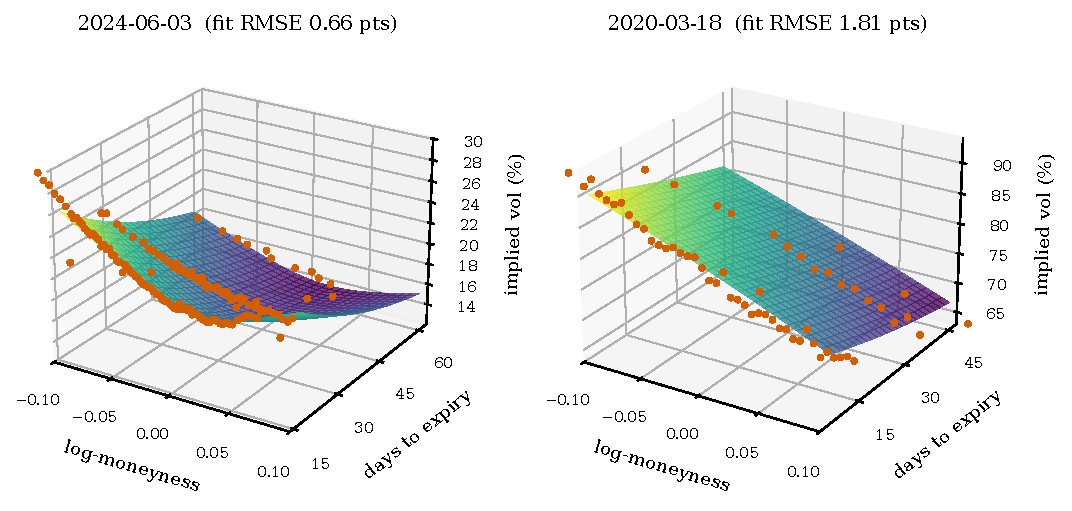
\includegraphics[width=\textwidth]{figures/surface3d}
\caption{Calibrated Heston implied-volatility surface (coloured) against market quotes (dots) on a calm day (\SurfDateA, left) and in the COVID-19 crash (\SurfDateB, right). Note the different vertical scales.}\label{fig:surface}
\end{figure}

\begin{figure}[ht]
\centering
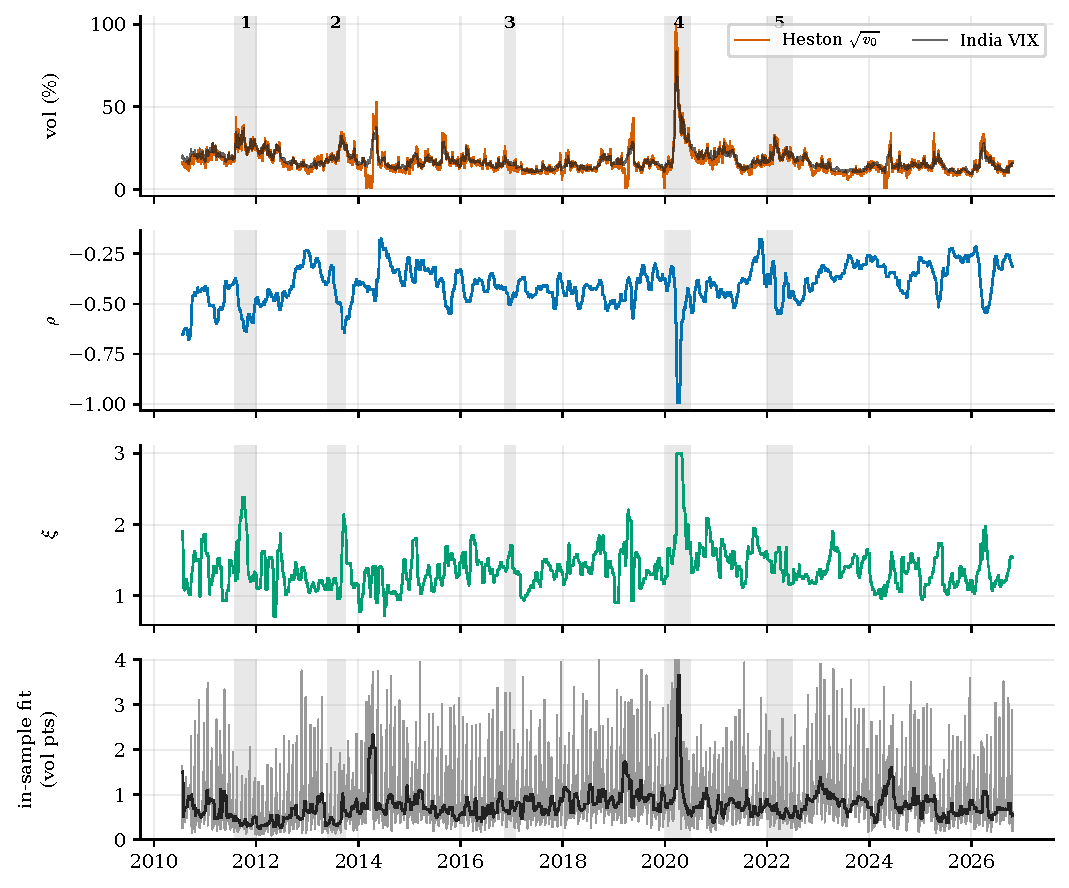
\includegraphics[width=\textwidth]{figures/params_ts}
\caption{Calibrated parameters (21-day rolling medians for $\rho,\xi$) and in-sample fit error. Grey bands are the five stress events of Table~\ref{tab:hedge}, in that order.}\label{fig:params}
\end{figure}

\begin{table}[ht]
\centering
\caption{Median calibrated parameters; ``$\kappa$ at bound'' is the share of days at the upper bound 15; fit RMSE in vol points.}\label{tab:params}
\begin{tabular}{lrrrrrr}
\toprule
Sample & $v_0$ & $\theta$ & $\xi$ & $\rho$ & $\kappa$ at bound & Fit RMSE \\
\midrule
Train 2010--18 & 0.026 & 0.028 & 1.31 & $-$0.42 & 62\% & 0.68 \\
Test 2019--26 & 0.021 & 0.024 & 1.38 & $-$0.37 & 79\% & 0.79 \\
COVID-19 crash & 0.095 & 0.076 & 1.94 & $-$0.49 & 33\% & 0.94 \\
All days & 0.023 & 0.026 & 1.34 & $-$0.40 & 70\% & 0.73 \\
\bottomrule
\end{tabular}

\end{table}

\emph{One-day-ahead pricing.} For each option quoted on consecutive days $(t,t+1)$ we price it on day $t+1$ using only day-$t$ information: Heston with day-$t$ parameters; Black--Scholes at the contract's own day-$t$ implied vol (``sticky strike'', the market benchmark); and Black--Scholes at the day-$t$ ATM vol (flat smile). Table~\ref{tab:pricing} and Figures~\ref{fig:oosyear}--\ref{fig:oossurf} show the results over \NOptionDays{} option-days. Heston removes most of the flat-volatility error in every year and away from the money, but never beats yesterday's own smile, which already contains each contract's previous price. Its excess error is concentrated in short-dated options far from the money, where a five-parameter model cannot follow the short-end skew.

\begin{table}[ht]
\centering
\caption{Experiment B: one-day-ahead pricing RMSE in implied-vol points. Last column: change in mean squared error of Heston relative to BS own vol.}\label{tab:pricing}
\begin{tabular}{lrrrrr}
\toprule
Sample & Option-days & BS flat & BS own & Heston & Heston vs BS own \\
\midrule
All days & 391\,792 & 3.87 & 1.11 & 1.55 & +94\% \\
Train 2010--18 & 110\,566 & 3.84 & 1.03 & 1.47 & +103\% \\
Test 2019--26 & 281\,226 & 3.89 & 1.14 & 1.58 & +91\% \\
Test, calm & 223\,069 & 3.87 & 0.85 & 1.35 & +154\% \\
Test, stress & 58\,157 & 3.95 & 1.88 & 2.25 & +43\% \\
COVID-19 crash & 6\,908 & 5.17 & 3.21 & 3.76 & +37\% \\
Test excl.\ COVID & 274\,318 & 3.85 & 1.04 & 1.48 & +104\% \\
\bottomrule
\end{tabular}

\end{table}

\begin{figure}[ht]
\centering
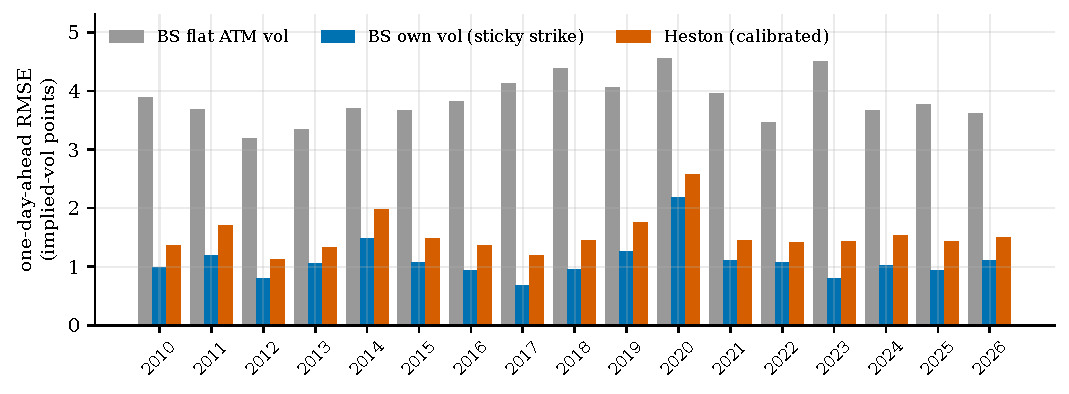
\includegraphics[width=\textwidth]{figures/oos_by_year}
\caption{One-day-ahead pricing RMSE by year: BS own $<$ Heston $<$ BS flat in every year.}\label{fig:oosyear}
\end{figure}

\begin{figure}[ht]
\centering
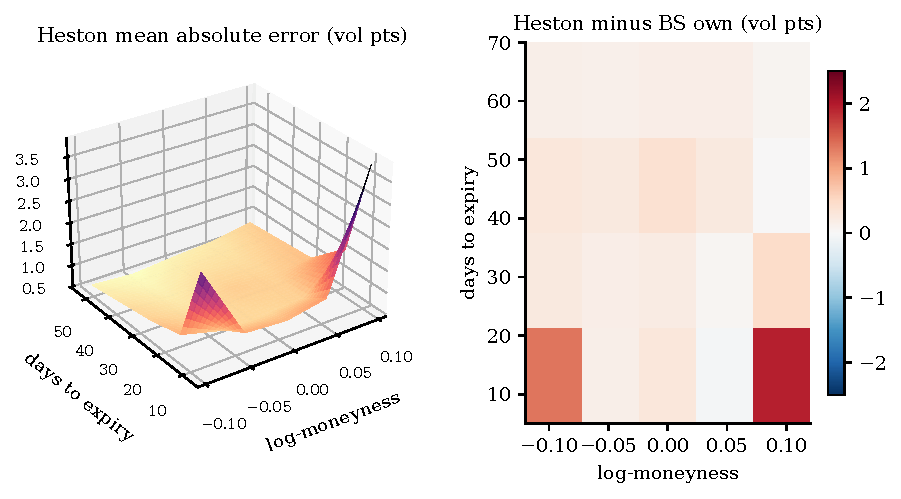
\includegraphics[width=\textwidth]{figures/oos_surface}
\caption{Left: Heston mean absolute error (test period) over moneyness and maturity. Right: its excess over BS own vol, concentrated in short-dated options in the wings.}\label{fig:oossurf}
\end{figure}

\emph{Hedging traded calls.} Each day we sell the monthly call nearest the money (about 21 trading days to expiry) and hedge it daily with the same-expiry future, with the Black--Scholes delta at the option's own implied vol, the Heston delta $C_F$, or the minimum-variance delta \eqref{eq:mv}. Costs are zero here. Comparisons are paired, with intervals from a block bootstrap over 21-day blocks of dates (Table~\ref{tab:hedge}, Figure~\ref{fig:hedgedist}).
In the test period the plain Heston delta \emph{increases} the hedging variance relative to Black--Scholes by $\HvsBSTest\%$ ($z=\HvsBSTestZ$); the correction in \eqref{eq:mv} repairs it ($\MVvsHTest\%$ against the plain Heston delta, $z=\MVvsHTestZ$), giving a tie with Black--Scholes ($\MVvsBSTest\%$, $z=\MVvsBSTestZ$; standard deviation \HedgeSDMV{} vs \HedgeSDBS{} bp, against \HedgeSDNone{} bp unhedged). The only significant gain is in the COVID window ($\MVvsBSCovid\%$, $z=\MVvsBSCovidZ$, \NCovid{} overlapping options in one episode); without it the difference is $\MVvsBSExCovid\%$ ($z=\MVvsBSExCovidZ$).

\begin{table}[ht]
\centering
\caption{Experiment B: hedging a short ATM monthly call daily with futures. None, BS, Heston, MV: standard deviation of the error in bp of $F_0$. Last two columns: paired change in variance relative to BS ($^*$: block-bootstrap $|z|\ge2$).}\label{tab:hedge}
\small
\begin{tabular}{lrrrrrrr}
\toprule
Sample & $n$ & None & BS & Heston & MV & Heston/BS & MV/BS \\
\midrule
All days & 3931 & 259 & 55.1 & 63.7 & 52.9 & +34\%$^{*}$ & $-$8\% \\
Train 2010--18 & 2058 & 254 & 48.7 & 55.8 & 50.0 & +31\%$^{*}$ & +5\% \\
Test 2019--26 & 1873 & 264 & 61.2 & 71.3 & 55.9 & +36\%$^{*}$ & $-$17\% \\
Test, calm & 1364 & 202 & 52.0 & 55.3 & 51.6 & +13\% & $-$1\% \\
Test, stress & 509 & 365 & 80.4 & 101.1 & 66.1 & +58\%$^{*}$ & $-$32\% \\
Test excl.\ COVID & 1760 & 235 & 51.1 & 58.2 & 53.1 & +30\%$^{*}$ & +8\% \\
US downgrade / Euro crisis & 101 & 327 & 41.6 & 60.0 & 38.5 & +108\%$^{*}$ & $-$14\% \\
Taper tantrum & 79 & 290 & 61.1 & 63.9 & 82.0 & +9\% & +80\% \\
Demonetisation & 59 & 281 & 35.8 & 33.5 & 45.3 & $-$13\% & +60\% \\
COVID-19 crash & 113 & 515 & 147.1 & 178.5 & 89.3 & +47\%$^{*}$ & $-$63\%$^{*}$ \\
2022 rate-hike sell-off & 123 & 279 & 65.5 & 84.2 & 62.1 & +65\%$^{*}$ & $-$10\% \\
\bottomrule
\end{tabular}

\end{table}

\begin{figure}[ht]
\centering
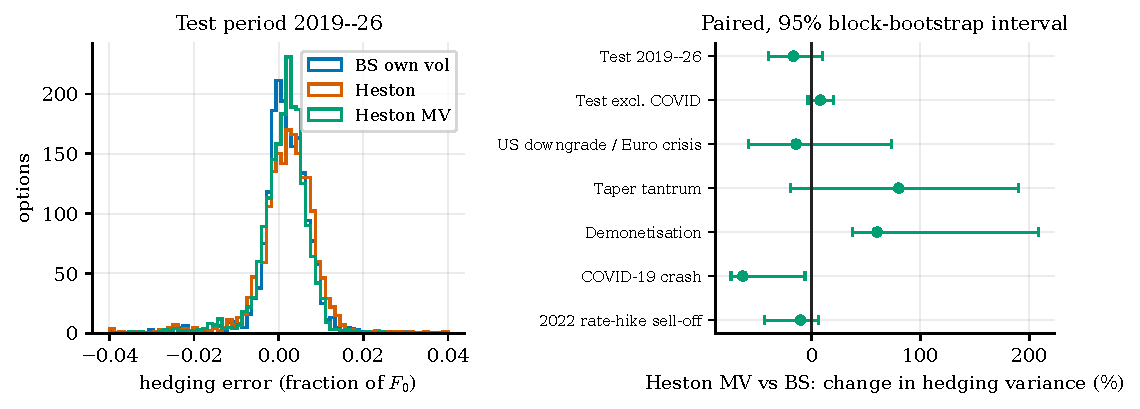
\includegraphics[width=\textwidth]{figures/hedge_dist}
\caption{Experiment B. Left: hedging errors in the test period. Right: change in hedging variance of the Heston minimum-variance hedge relative to BS, with 95\% block-bootstrap intervals.}\label{fig:hedgedist}
\end{figure}

\heading{7. Simulation: what would theory predict?}
\noindent The real-data hedging gains are small. Is that because the minimum-variance hedge is not useful, or because NIFTY is not Heston? We answer it by simulating a world in which Heston is exactly true. We simulate 10\,000 paths of \eqref{eq:heston} under $\Q$ (full-truncation Euler, 20 steps per day; Lord et al.\ 2010), sell an ATM call with 21 trading days to expiry at its Heston price, and hedge it with the Black--Scholes delta at the option's own implied volatility, the Heston delta and the minimum-variance delta, rebalancing four times a day, daily, every two days or weekly. All hedges see the same paths, so comparisons are paired. We use two parameter sets: the median of our daily calibrations, $\SimCalParams$, and the team's time-series estimate (low vol-of-vol).

\emph{Results} (Table~\ref{tab:sim}, Figure~\ref{fig:sim}). Even when the model is exactly right, the minimum-variance hedge lowers the daily hedging variance relative to the Black--Scholes own-vol hedge by only $\SimCalMVvsBS\%$ (calibrated) and $\SimTSMVvsBS\%$ (time-series), while the plain Heston delta is \emph{worse} by $\SimCalHvsBS\%$ and $\SimTSHvsBS\%$. This is the same ordering as on real NIFTY (Table~\ref{tab:hedge}). The reason is that the option's own implied volatility already carries the skew, so the Black--Scholes own-vol delta is close to optimal; the Heston delta, which holds variance fixed, misses the spot--volatility correlation, and the term $\rho\xi C_v/F$ puts it back. A gain of a few percent is far too small to detect with about 1\,900 overlapping real options, so the real-data ``tie'' is what theory predicts, not a failure of the method.

The rebalancing interval tells the second half of the story. With low vol-of-vol (time-series parameters) the error falls from \SimTSMVWeek{} bp (weekly) to \SimTSMVFour{} bp (four times a day): most risk is discretisation error, which more trading removes, as in Black--Scholes. With the calibrated vol-of-vol it only falls from \SimCalMVWeek{} to \SimCalMVFour{} bp: a large floor remains however often we trade. That floor is the volatility risk that futures cannot hedge, the incompleteness of Section~2, made visible.

\begin{table}[ht]
\centering
\caption{Simulated Heston world: standard deviation of the hedging error (bp of $F_0$) by rebalancing interval, and paired change in variance relative to the BS own-vol hedge at daily rebalancing (95\% bootstrap interval). 10\,000 common paths, no costs.}\label{tab:sim}
\small
\begin{tabular}{llrrrrr}
\toprule
Parameters & Hedge & 4/day & 1 day & 2 days & 5 days & Var.\ vs BS (daily) \\
\midrule
Calibrated & BS own vol & 75.3 & 81.1 & 88.2 & 104.8 & -- \\
 & Heston delta & 79.1 & 85.0 & 92.8 & 110.7 & +10\% [+9, +11] \\
 & Heston MV & 73.9 & 79.2 & 85.9 & 102.4 & $-$5\% [$-$6, $-$4] \\
\midrule
Time-series & BS own vol & 30.8 & 45.4 & 57.8 & 84.7 & -- \\
 & Heston delta & 33.3 & 47.1 & 59.5 & 86.1 & +8\% [+7, +9] \\
 & Heston MV & 30.2 & 44.8 & 57.3 & 84.1 & $-$2\% [$-$3, $-$2] \\
\bottomrule
\end{tabular}

\end{table}

\begin{figure}[ht]
\centering
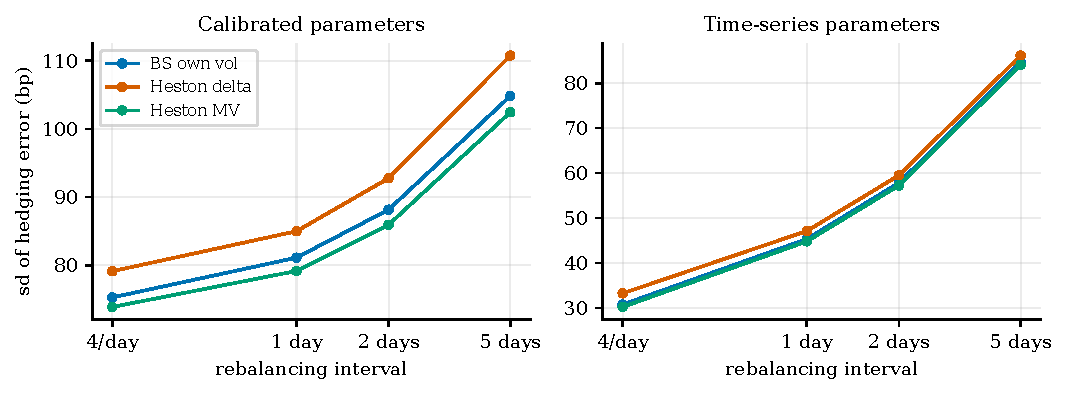
\includegraphics[width=\textwidth]{figures/simulation}
\caption{Simulated Heston world: hedging error against rebalancing interval. Left: calibrated parameters (high vol-of-vol), where a floor of unhedgeable volatility risk remains. Right: time-series parameters, where frequent rebalancing removes most of the error.}\label{fig:sim}
\end{figure}

\FloatBarrier
\heading{8. From the project to a trading strategy: selling hedged insurance.}
\noindent \emph{The everyday idea.} An index call option is insurance: the buyer pays a premium now and is paid if the market rises above the strike. As with car or health insurance, buyers on average pay more than the expected payout; in options this margin is the \emph{volatility risk premium}. An insurer earns it by selling many policies and keeping its risk under control. The option seller can do the same, and the project tells it how to control the risk: hedge the market direction with futures using the delta of Sections~2--3.

\emph{The strategy} (uses only information at each day's close). Every trading day, sell one ATM monthly NIFTY call sized at $1/21$ of the book, so about one month of options is always open; hedge each option daily with the same-expiry future using (a) no hedge, (b) the Black--Scholes delta, or (c) the Heston minimum-variance delta \eqref{eq:mv}; hold to expiry. A simple risk rule, \emph{skip stress}, opens no new option on days the causal India VIX label signals stress. The book is valued every day (mark-to-market): each open option at Black-76 with its own market implied volatility (in the last week before expiry, where our data filter has no quotes, the volatility is held at its last quoted value), and the futures at their close; summed over its life, an option's daily profit equals its final result. Costs are a futures fee per unit traded and half the option bid--ask spread: low (1 bp, 1\% of premium) or high (5 bp, 3\%). Rules and costs were fixed in advance, not fitted.

\emph{A worked trade.} On \ExDate{} the future is at \ExF{} and we sell the \ExK{} call expiring \ExExpiry{} for \ExPrem{} index points. \ExStory{} the net result is \ExNet{} points (\ExNetBp{} bp of notional), the median outcome (before costs) of the MV-hedged trades in the test period. Most of the market move is offset by the hedge, and what remains is the insurance margin.

\emph{Results.} The average premium is \StratPremium{} bp of notional. Before costs a hedged option earns on average \StratMeanGrossBS{} bp (BS hedge) or \StratMeanGrossMV{} bp (Heston MV), while the unhedged seller \emph{loses} \StratMeanNoneAbs{} bp, because NIFTY rose strongly over the period. Table~\ref{tab:strategy} and Figure~\ref{fig:strategy} show the book in the 2019--26 test period. With low costs the BS-hedged book returns \StratBSRet\% of notional a year with Sharpe ratio \StratBSSharpe{} and maximum drawdown \StratBSDD\%; the Heston-MV-hedged book returns \StratMVRet\% with Sharpe \StratMVSharpe{} and a smaller drawdown, \StratMVDD\%. The unhedged book returns \StratNoneRet\% with a drawdown of \StratNoneDD\%. With high costs the edge disappears (\StratBSHighRet\% and \StratMVHighRet\% a year). The skip-stress rule lowers risk but also returns, because insurance is most expensive exactly in stress (Sharpe \StratMVSkipSharpe{} for the MV book).

\emph{What it teaches.} (i) Hedging turns a losing directional bet into a steady small earner; (ii) the Heston hedge derived in this project has smaller drawdowns than the Black--Scholes hedge for a similar return, which is what an insurer cares about, though its Sharpe ratio is slightly lower and its worst single day is a little worse (\StratMVWorstDay\% against \StratBSWorstDay\% of notional); (iii) whether it makes money at all is decided by execution costs; (iv) the gains are small per unit of notional (a trader would scale them with margin and leverage, which also scales the losses), and they come with crash risk (shaded COVID band). We present it as a demonstration, not investment advice.

\begin{figure}[ht]
\centering
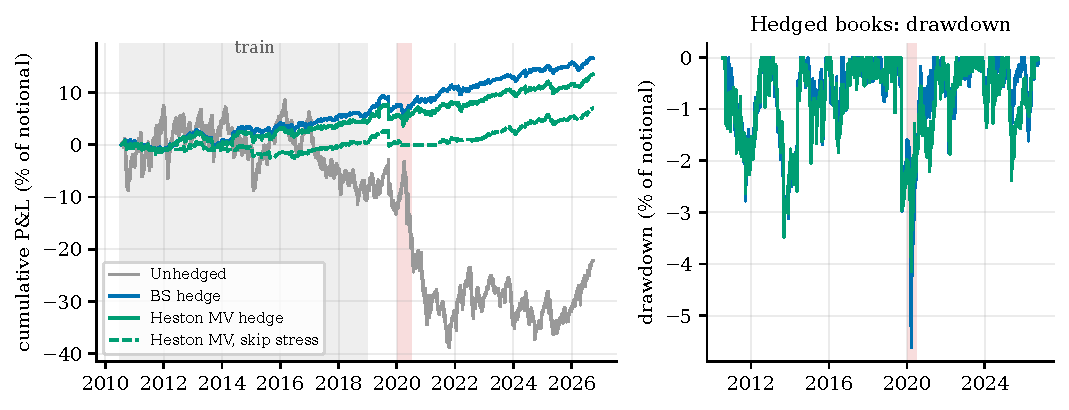
\includegraphics[width=\textwidth]{figures/strategy}
\caption{Selling one hedged ATM monthly call per day, low costs. Left: cumulative P\&L in \% of book notional (grey: training period; red band: COVID-19). Right: drawdown of the two hedged books.}\label{fig:strategy}
\end{figure}

\begin{table}[ht]
\centering
\caption{Strategy performance in the test period 2019--26 (\% of notional per year; Sharpe without risk-free rate; Max DD and worst day in \% of notional, from daily mark-to-market). The last column is the Sharpe ratio on the training period 2010--18.}\label{tab:strategy}
\small
\begin{tabular}{lllrrrrrr}
\toprule
Costs & Hedge & Entry rule & Return/yr & Vol/yr & Sharpe & Max DD & Worst day & Sharpe (train) \\
\midrule
Low & Unhedged & every day & $-$1.79 & 8.33 & $-$0.21 & $-$36.0 & $-$4.39 & $-$0.13 \\
 & Unhedged & skip stress & +2.04 & 5.33 & 0.38 & $-$11.9 & $-$3.31 & $-$0.37 \\
 & BS hedge & every day & +1.41 & 1.91 & 0.74 & $-$5.6 & $-$2.18 & 0.45 \\
 & BS hedge & skip stress & +0.78 & 1.28 & 0.61 & $-$3.0 & $-$2.18 & 0.11 \\
 & Heston MV hedge & every day & +1.20 & 1.93 & 0.62 & $-$4.1 & $-$2.47 & 0.33 \\
 & Heston MV hedge & skip stress & +0.88 & 1.37 & 0.64 & $-$3.0 & $-$2.47 & 0.04 \\
\midrule
High & Unhedged & every day & $-$2.21 & 8.33 & $-$0.27 & $-$37.1 & $-$4.39 & $-$0.18 \\
 & Unhedged & skip stress & +1.79 & 5.33 & 0.34 & $-$12.2 & $-$3.31 & $-$0.41 \\
 & BS hedge & every day & +0.17 & 1.93 & 0.09 & $-$6.6 & $-$2.21 & $-$0.32 \\
 & BS hedge & skip stress & $-$0.07 & 1.30 & $-$0.06 & $-$4.1 & $-$2.21 & $-$0.61 \\
 & Heston MV hedge & every day & $-$0.03 & 1.95 & $-$0.02 & $-$4.9 & $-$2.51 & $-$0.42 \\
 & Heston MV hedge & skip stress & +0.04 & 1.39 & 0.03 & $-$3.6 & $-$2.51 & $-$0.66 \\
\bottomrule
\end{tabular}

\end{table}

\FloatBarrier
\heading{9. Discussion and limitations.}
\noindent The two experiments agree on the hedging question: the minimum-variance correction $\rho\xi C_v/F$ matters, because without it a stochastic-volatility delta is worse than Black--Scholes; with it the hedge ties Black--Scholes and helps mainly in a crash, where it also lowers tail losses. They differ on pricing because they answer different questions: with only historical inputs, a model that captures the skew (rough Heston) beats a flat VIX volatility, while with daily calibration even a good model cannot beat the market's own previous-day smile.
\begin{compactitem}
\item \textbf{One market.} Only NIFTY; we found no free, verifiable historical option chains for other markets.
\item \textbf{Data.} Daily closes of options, futures and VIX are not synchronous; India VIX is a 30-day average used as a variance proxy.
\item \textbf{Models.} European options only. In Experiment B, $\kappa$ is not identified. The rough Heston pricer is numerically fragile at short maturities, and it was not calibrated daily to option chains.
\item \textbf{Hedging.} Experiment A uses synthetic options priced at India VIX; Experiment B ignores costs. Futures-only hedges; no hedging with other options.
\item \textbf{Statistics.} Events are few, option lives overlap, and many comparisons are made, so a lone $|z|\approx2$ is weak evidence.
\item \textbf{Simulation check.} In the rough Hawkes--Heston model with jumps, the stock-only projection hedge has a 99\% shortfall of \TSSimGKW{} bp against \TSSimBS{} bp for Black--Scholes, so the model's own hedge is better inside the model; the real-data gains above are much smaller.
\end{compactitem}

\heading{10. Conclusion.}
\noindent Stochastic and rough volatility describe NIFTY options much better than constant volatility: calibrated Heston has \PriceFlatOverHeston{} times smaller pricing error than a single-volatility Black--Scholes, and rough Heston prices traded options best when only historical inputs are available. For hedging, the important ingredient is the minimum-variance correction derived from Itô's formula: it turns a poor stochastic-volatility delta into one that matches Black--Scholes, with a clear advantage only in the COVID-19 crash. A simulation shows that this is what theory predicts: the gain of the optimal hedge over a Black--Scholes delta at the option's own implied volatility is only a few percent even when the model is true, and with high vol-of-vol a floor of unhedgeable volatility risk remains however often one trades. As a practical application, selling hedged options harvests the volatility risk premium: hedging turns a losing directional bet into a small steady return, the Heston hedge reduces drawdowns, and trading costs decide whether anything is left. The evidence does not support a large tradable advantage over the market-implied Black--Scholes hedge in normal markets.

\heading{References.}
\begin{compactenum}[\small 1.]
\item {\small F.\ Black, M.\ Scholes, The pricing of options and corporate liabilities, \emph{J.\ Polit.\ Econ.} 81 (1973) 637--654.}
\item {\small R.\ C.\ Merton, Theory of rational option pricing, \emph{Bell J.\ Econ.\ Manag.\ Sci.} 4 (1973) 141--183.}
\item {\small S.\ Heston, A closed-form solution for options with stochastic volatility with applications to bond and currency options, \emph{Rev.\ Financ.\ Stud.} 6 (1993) 327--343.}
\item {\small H.\ Albrecher, P.\ Mayer, W.\ Schoutens, J.\ Tistaert, The little Heston trap, \emph{Wilmott} (2007) 83--92.}
\item {\small J.\ Gil-Pelaez, Note on the inversion theorem, \emph{Biometrika} 38 (1951) 481--482.}
\item {\small O.\ El Euch, M.\ Rosenbaum, Perfect hedging in rough Heston models, \emph{Ann.\ Appl.\ Probab.} 28 (2018) 3813--3856.}
\item {\small O.\ El Euch, M.\ Rosenbaum, The characteristic function of rough Heston models, \emph{Math.\ Finance} 29 (2019) 3--38.}
\item {\small J.\ Gatheral, T.\ Jaisson, M.\ Rosenbaum, Volatility is rough, \emph{Quant.\ Finance} 18 (2018) 933--949.}
\item {\small J.\ Hull, A.\ White, Optimal delta hedging for options, \emph{J.\ Banking Finance} 82 (2017) 180--190.}
\item {\small R.\ Lord, R.\ Koekkoek, D.\ van Dijk, A comparison of biased simulation schemes for stochastic volatility models, \emph{Quant.\ Finance} 10 (2010) 177--194.}
\item {\small Y.\ Wang, X.\ Wang, Variance-optimal hedging in the rough Hawkes--Heston model, arXiv:2609.08541 (2026); code at github.com/gagawjbytw/hedging\_rough\_hawkes\_heston.}
\item {\small S.\ Shreve, \emph{Stochastic Calculus for Finance II}, Springer, 2004.}
\item {\small NSE India: F\&O bhavcopy archives and India VIX; NSE Indices: NIFTY 50 history.}
\end{compactenum}

\bigskip
% Public builds define \PublicBuild to force the names-only list.
\noindent\begin{minipage}{\textwidth}   % keeps the heading with its table
\ifdefined\PublicBuild
\noindent\textbf{Group members.}\par
\begin{center}
\renewcommand{\arraystretch}{1.25}
\begin{tabular}{|c|p{5cm}|}
\hline
\textbf{No.} & \textbf{Name} \\ \hline
1 & Dhyan Laad \\ \hline
2 & Natasha Nalwaya \\ \hline
3 & Shrirang Bhale \\ \hline
4 & Tanmai Chekuri \\ \hline
5 & Shivam Mahto \\ \hline
\end{tabular}
\end{center}

\else
\IfFileExists{members.tex}{\input{members}}{\noindent\textbf{Group members.}\par
\begin{center}
\renewcommand{\arraystretch}{1.25}
\begin{tabular}{|c|p{5cm}|}
\hline
\textbf{No.} & \textbf{Name} \\ \hline
1 & Dhyan Laad \\ \hline
2 & Natasha Nalwaya \\ \hline
3 & Shrirang Bhale \\ \hline
4 & Tanmai Chekuri \\ \hline
5 & Shivam Mahto \\ \hline
\end{tabular}
\end{center}
}
\fi
\end{minipage}

\end{document}
